\begin{frame}
  \frametitle{\problemtitle}

  \begin{columns}
    \column{0.73\linewidth}
    \begin{description}
      \item<+->[Problem:] Given a tree of $n$ vertices, remove $k$ of them to
        minimize the number of remaining leaves.
      \item<+->[Insight:] Removing a leaf only reduces the count if it has siblings.
      \item<+->[Greedy:] Repeatedly remove the shortest \emph{leaf-branch}.
      \item<+->[Insight:] Below each vertex, the deepest path is always
        removed last.
      \item<+->[Solution:] Using DFS or bottom-up DP, find the length of the
        deepest path below each node.
      \item<+->[] At each node, increase the length of the deepest child by one,
        and mark the other children's paths as final (bold).
      \item<+->[] Sort the final lengths ($[1,1,2,5]$), and count how many of them sum
        to at most $k$.
      \item<+->[Run time:] $\mathcal O(n)$.
    \end{description}

    \column{0.27\linewidth}

    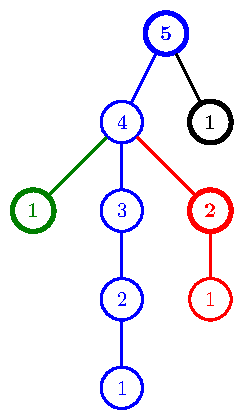
\includegraphics[width=\linewidth]{solution-figure.pdf}
  \end{columns}

  \solvestats
\end{frame}
